\documentclass[12pt]{article}

% import a set of useful packages for math
\usepackage{amsmath, amsfonts, amssymb}

% this package makes margins smaller
\usepackage{fullpage}

% for importing images
\usepackage{graphicx}

%%%% import any other packages here
\usepackage{algorithm}
\usepackage[noend]{algpseudocode}
\usepackage{pythonhighlight}
\usepackage{listings}
\usepackage{pdfpages}
%%%% make any other definitions here


%%%%%%%%%%%%%%%%%%%%%%%%%%%%%%%%
\begin{document}
%%%%%%%%%%%%%%%%
\section*{Why we tried this}
The seq2seq model used resembles the one mention in the paper (https://arxiv.org/pdf/1409.3215.pdf). While this architecture is usually used for language translation, it happens to also be widely used for chat bot creation. The sucess the seq2seq model has had in other chatbot implementations we researched, along with it's easy implementation in Keras is why this architecture was chosen.

\section*{Data Preparation}
\begin{itemize}
  \item The first decision made involved how to split text into tokens. For the english language the best way to split words is on space so this is what was done to extract tokens from a chunk of text.
  \item The next step involved removing all numeric data. This was done using a simple regular expression.
  \item The next problem was to deal with punctuation's. This problem was handled by treating each certain punctuation's as as separate tokens. A select number of punctuation's were kept and a space was added between the word and the punctuation thereby turning the punctuation into a token
\end{itemize}
\begin{python}
    keepPunct = '[.,!?;]'
    re.findall(r"[\w]+|"+keepPunct, 
            'This is a test. Is this test 2?')
    >>['This','is','a','test','.','Is','this','test','?']
\end{python}

\begin{itemize}
    \item When the sentence being processed is an output sentence a start and end token are added to the sentence.
\end{itemize}
\begin{python}
    >>['<START> This is a test . Is this test ? <END>']
\end{python}
\begin{itemize}
    \item To make word data ingestible by the embedding layer and easier to work with in general, every word was mapped to a numeric token. The \textbf{tokenizer} consumed the entire corpus and creates a dictionary of word to token maps. The tokeinzer was then used to convert every word (split on space) in the input and output sentences to their tokenized equivalent.
\end{itemize}
\begin{python}
    tokenizer = keras.preprocessing.text.Tokenizer(filters='\t\n',
                                                   oov_token='<UNK>', 
                                                   lower=False)
    tokenizer.fit_on_texts(inputs + outputs)
    tokenizer.texts_to_sequences(['This is a test input .',
                        '<START> This is another test output . <END>'])
    >>[[1,2,3,4,5,8],[10, 1, 2, 6, 4, 7, 8, 11]]
\end{python}
\begin{itemize}
    \item The next step involved \textbf{padding} the tokenized sequences so they have the same size during model training. This was done by finding the longest sequence and padding all other sequences with zeros to have the same length as the longest sequence. The input sequence were pre padded while the output was post padded.
\end{itemize}
\begin{python}
    inputSequences = [[1,2,4,8],[2,4,3]]
    ouputSequences = [[10, 1, 2, 6, 11], [10, 1, 2, 11]]
    paddedInputs = preprocessing.sequence.pad_sequences(inputSequences,
                                                     maxlen=maxInputLen,
                                                     padding='pre' )
    paddedOutputs = preprocessing.sequence.pad_sequences(ouputSequences,
                                                     maxlen=maxOutputLen,
                                                     padding='post' )
    paddedInputs
    >>[[1,2,4,8],[0,2,4,3]]
    paddedOutputs
    >>[[10, 1, 2, 6, 11], [10, 1, 2, 11,0]]
\end{python}
\begin{itemize}
    \item Every token in the sequence had to be given a unique vector representation (https://papers.nips.cc/paper/5021-distributed-representations-of-words-and-phrases-and-their-compositionality.pdf). This was handle by the \textbf{keras.layers.Embedding} layer. To provide contextual representations of words (tokens), \textbf{GloVe 300-dimensional word embeddings} were used to initialized the embedding layer weights. 
    \item Since the model outputs a softmaxed prediction on each word, the next step involved converting output tokens to \textbf{one-hot vectors}. Since the goal of the decoder was to predict the next token given the current token, the tokenized output sequence was shifted to the left by one step before being converted to one-hot vectors.  
\end{itemize}
\begin{python}
    #If the vocabulary was of size 3
    paddedOutputs = [1,2,3,0]
    paddedOutputs = paddedOutputs[1:] #left shift step
    onehotOutput = keras.utils.to_categorical( paddedOutputs , 3+1)
    onehotOutput
    >>[[0,1,0,0],[0,0,1,0],[0,0,0,1],[1,0,0,0]]
\end{python}

\section*{The Model}
\begin{center}
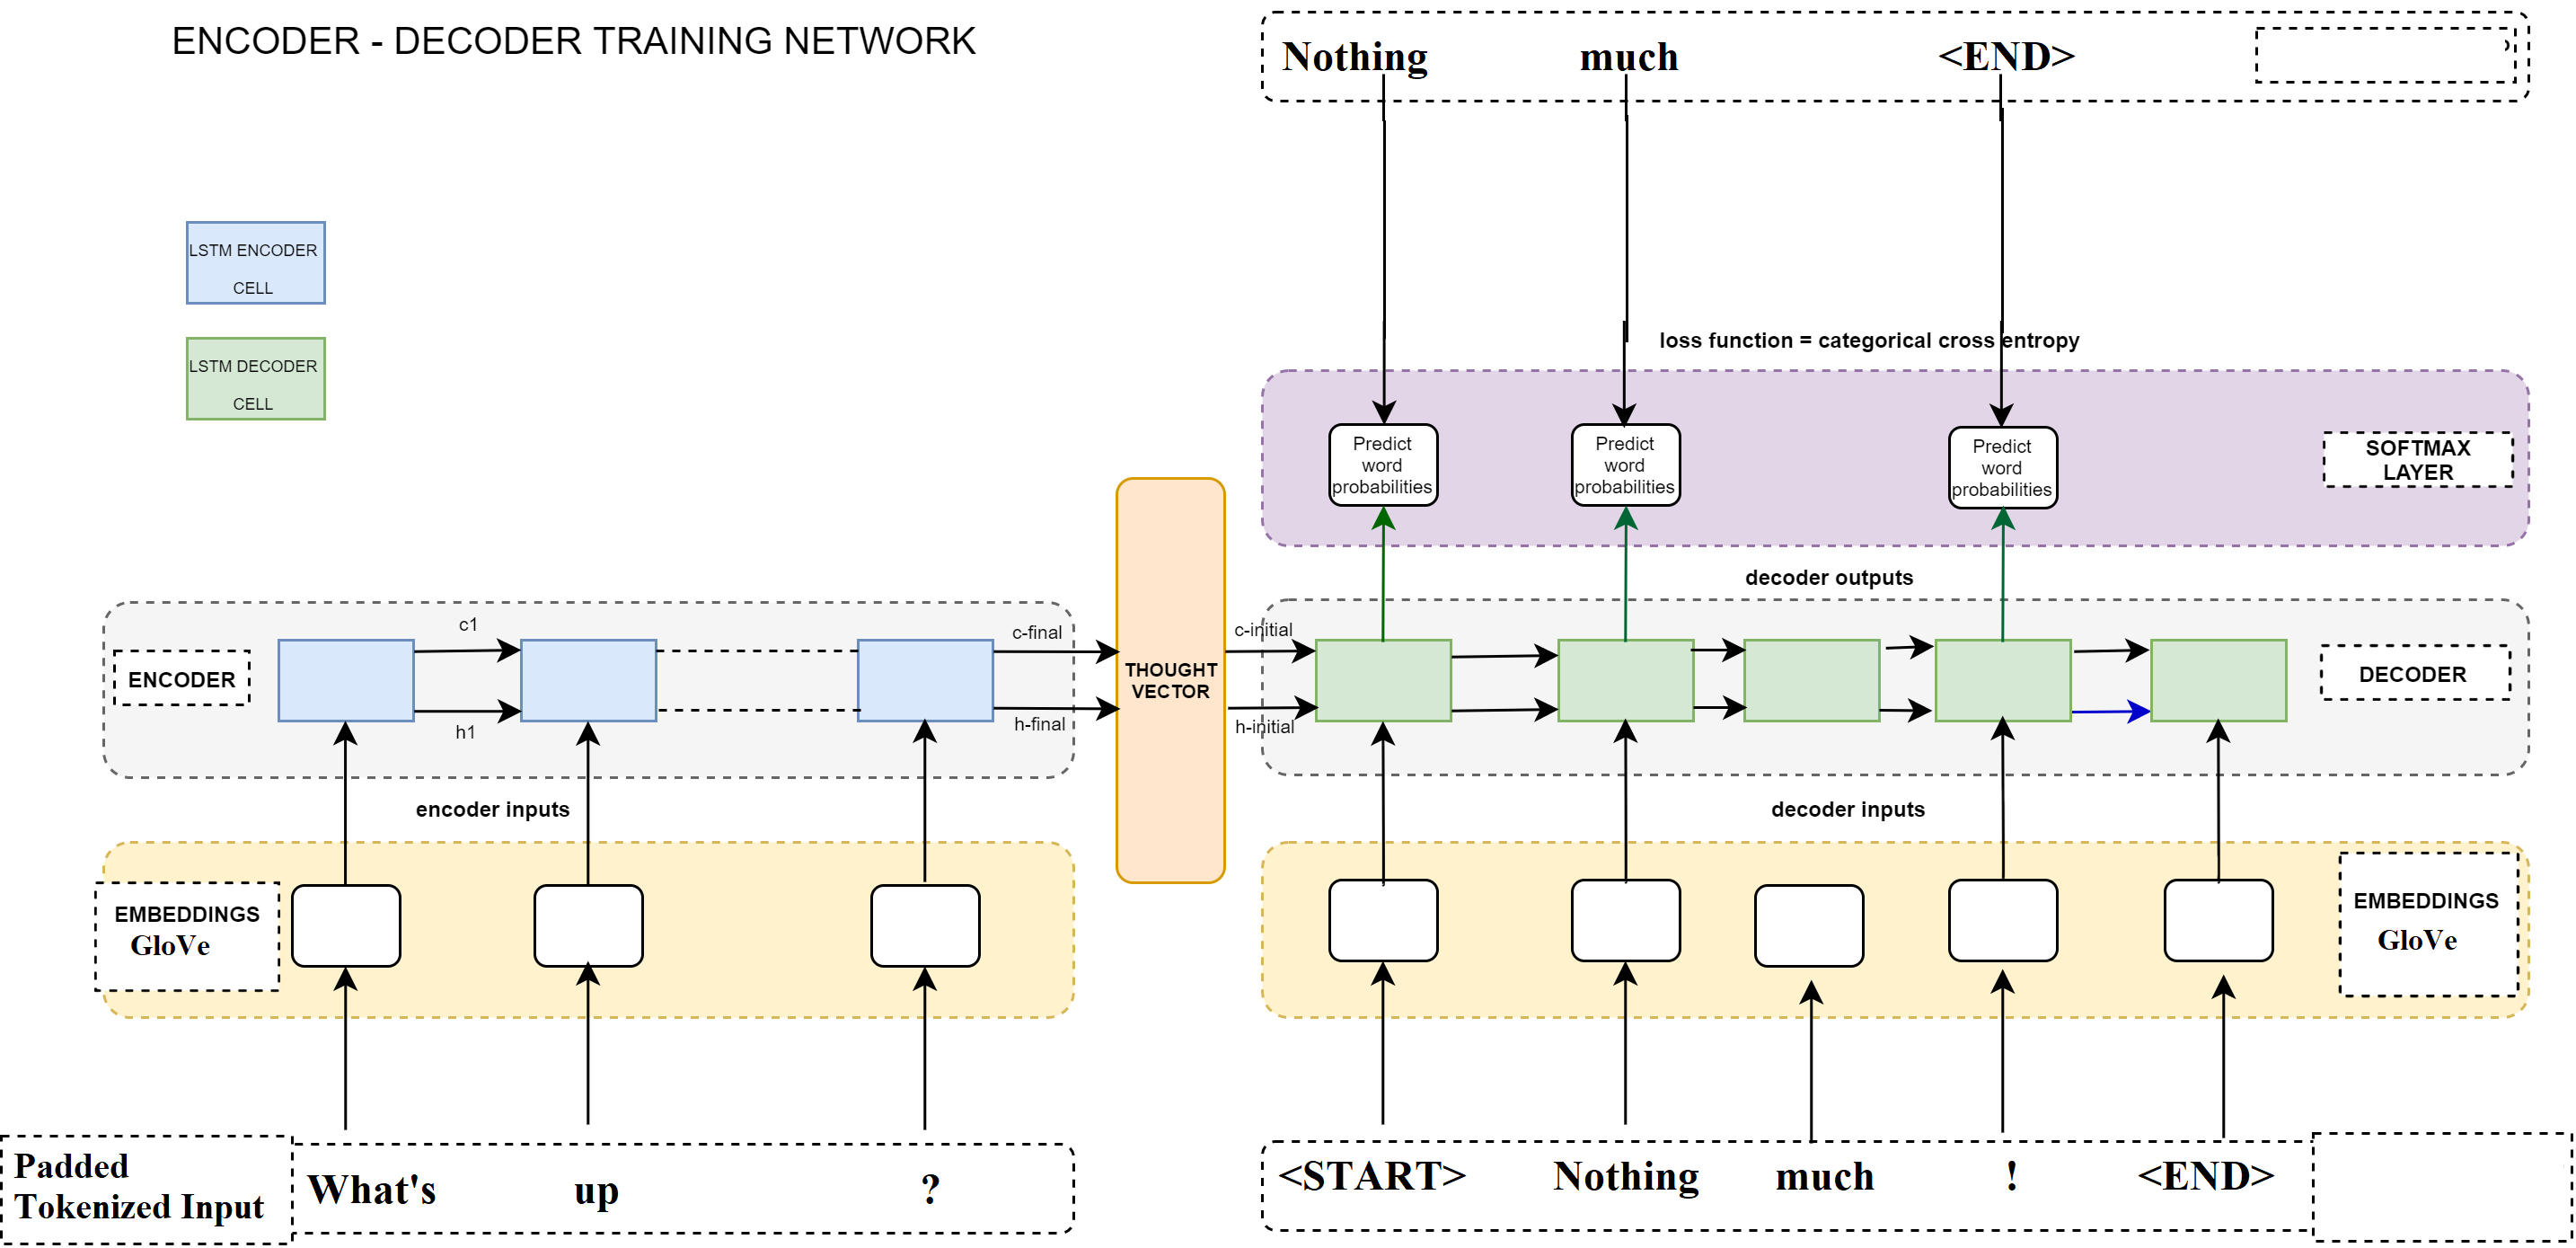
\includegraphics[width=160mm]{seq2seqModel.png}
\end{center}
\begin{itemize}
    \item The model consists of an Encoder and a Decoder.
    \item Padded input token sequences are converted to word embeddings using a\\ \textbf{Keras.embedding.layer}.
    \item  Word vectors are fed to the \textbf{keras.layers.LSTM} encoder LSTM one word at a time. The encoder LSTM tries to capture the essence of the encoder input sequence in two thought vectors, \textbf{the output context vector} and \textbf{the hidden state vector} that are passed to the decoder.
    \item The decoder LSTM, is fed padded output sequence word embeddings and two thought vectors, \textbf{the output context vector} and \textbf{the hidden state vector}. The decoder model is trained to use a dense SoftMax output layer \textbf{keras.layers.Dense} with activation \textbf{keras.activations.softmax} to predict the most probable output word among all words in the vocabulary.
    \item Once  the model is trained, an inference encoder and decoder model is created using the trained model weights. The inference encoder model takes in a user input question and generated two state vectors. The input state vectors are fed into the inference decoder model along with a sentence $<START>$ token. All words predicted by the SoftMax layer are captured until an $<END>$ token is generated. 
\end{itemize}

\begin{center}
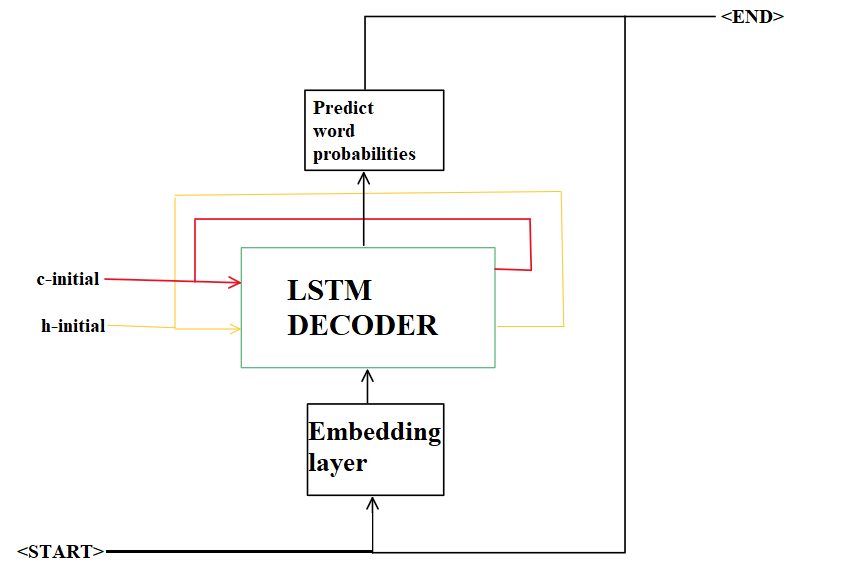
\includegraphics[width=160mm]{inference.png}
\end{center}

\section*{Pitfalls}
\begin{itemize}
    \item A major pitfall faced was during training the model. Specifically in providing the model with one-hot output vectors. As discussed above, the model uses a output sofmax layer to predict the best possible word output. This means the length of each training output vector equals the length of vocabulary. This is multiplies by the number of tokens (words) in the sequence and this is then multiplied by the number of training data points. With a vocabulary size of 3000 and a sequence length of 100 and training data size of 7000 the size of the entire output training data become $3000*100*7000$. This is too large an matrix to store. This problem was fixed by training in batches using a generator to generate batches of data for training instead on the entire data set. This was implemented using the Keras $fit\_generator$ function along with a custom data generation function. 
    \item The initial model randomly generated embedding vectors of tokens. This did give good results as the word embedding held no information regarding the tokens they represented. This problem was fixed using GloVe word embedding that contextually represented the words they were associated to.
    \item During development, while training on a large number of epochs, a singel failure in training lead to the loss of all training progress as the model was saved only in the end of training. This was fixed by creating a callback to save the model every specified number of epochs.
\end{itemize}

\section*{Future improvements}
\begin{itemize}
    \item While the current model seems to learn Joey like responses, it fails to understand how English sentences are structured. This leads to a lot of sentences failing tests as they are eliminated for not looking like english sentences. This can be fixed by adding a \textbf{Conditional Random Field (CRF)} layer using the Viterbi algorithm to give the model a sense of English sentence structure. This way a model know that an adverb comes after a verb etc. thereby facilitating the generation of English like sentences.
    \item The model currently takes an argmax of the output predictions to choose the most probable word. Using a \textbf{beam search} across predictions instead of just an argmax could improve prediction results.
    
    \item The current model used just two fixed length vectors to represent the entire input sequence. When input sequence are really long, two fixed length vectors may not be enough to capture its entire essence. Attention could help solve this issue. The technique was tried but could not be successfully implemented due to the time constraint. Adding attention to seq2seq models has been show to drastically improve performance of the model when the input sentences are long.
\end{itemize}


$*****************************************************************************$
\section*{Dataset}
To create the personality based chatbot, there was a need for a personality to mimic. For this personality data, TV show characters were chosen. This was done because the writer of TV shows develop a characters personality over many seasons that span multiple years. This gives each character a distinct personality that could be mimicked in a chatbot. Movies characters were not chosen as the character development is much shorter in a movie that is a few hours long. TV show transcripts also offer a larger dataset.\\

For this project, F.R.I.E.N.D.S was chosen as the TV show and Joey Tribbiani was chosen as the character. Joey was chosen as the character to study as he has a distinctive personality in the show. For those not familiar the show, Joey can be described as naive, sarcastic, loving, misogynistic and loud. \\

The data set was retrieved from: (https://fangj.github.io/friends/). The scrips were split up by episodes with a single episode's cvs file holding the script for that episode. Each script indicated the character speaking and the dialogue they spoke.
\begin{center}
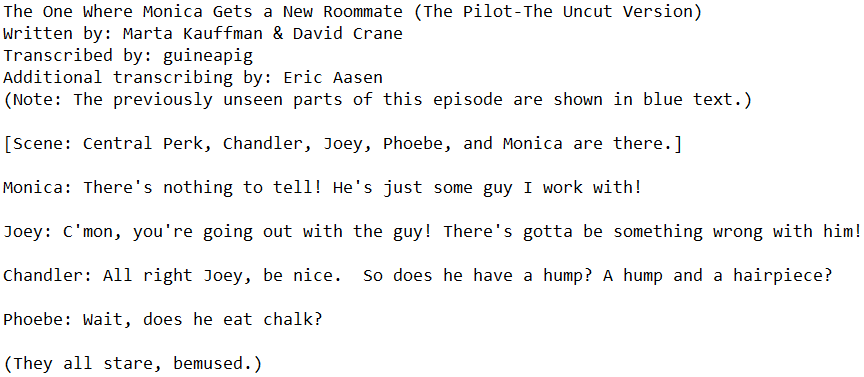
\includegraphics[width=160mm]{rawData.PNG}
\end{center}

The raw script was parsed to extract statement response pairs from each scene. We then collected all pairs where Joey was the responder. This was done using a python script that pulls keeps track of the previous character that was speaking. If the current character speaking is found to be Joey, the previous character's dialogue is saved as input and the current character's (Joey's) dialogue is saved as output. If the current character speaking is not joey the previous character becomes the current character and the algorithm moves on to the next dialogue. This is run across all episode scripts to extract training data. This extraction resulted in around 7000 training data points.
\begin{center}
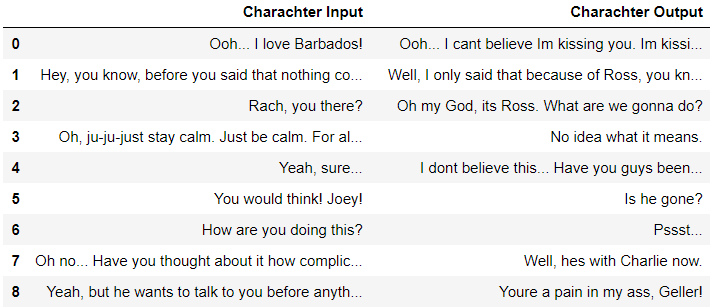
\includegraphics[width=160mm]{charachterData.PNG}
\end{center}

In additional to having Joey like personalities, we wanted our chatbot to in general respond like a human. To this end we considered pretraining our models on an additional dataset of general question and answer pairs. The goal of introducing this data set was to help the model understand generic a question answering format. Around 500 generic data points were used for training. We reserved 20 percent of both datasets to be used as testing data.
\begin{center}
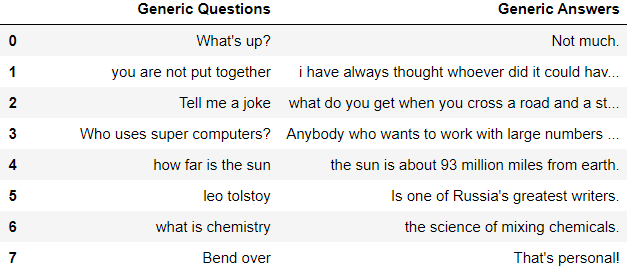
\includegraphics[width=160mm]{genericData.PNG}
\end{center}

\section*{Possible improvements}
In the data extraction section above it was mentioned that every dialogue uttered right before joey spoke was considered input for Joey and Joeys response was considered output. As a result of this, every time a person spoke, regardless of weather Joey heard it or not, Joeys dialogue said right after this is considered output. This means if Monica says something unrelated across the room and Joey responds to something on the television, it is still considered an input output pair. Eliminating this problem by implementing a better extraction algorithm could lead to a better data set. \\

Another possible way to augment the data set would be to increase the number of generic data the model is trained on. This would help give the model a better understanding of how questions need to be answered.
\end{document}